\documentclass[12pt]{article}
\usepackage{amsmath,amssymb,amsthm}
\usepackage{fullpage}
\usepackage{graphicx}
\usepackage{hyperref}
\usepackage{listings}

\theoremstyle{definition}
\newtheorem{thm}{Theorem}[section]
\newtheorem{lem}[thm]{Lemma}
\newtheorem{defn}{Definition}[section]
\newtheorem{conj}{Conjecture}[section]
\newtheorem{prob}{Open problem}[section]
\newcommand{\floor}[1]{\left\lfloor #1 \right\rfloor}
\newcommand{\ceil}[1]{\left\lceil #1 \right\rceil}
\newcommand{\bigC}[0]{\mathcal{C}}
\begin{document}
\emergencystretch 3em
\title{How hard is it to detect {\em some} cliques?}

\author{Josh Burdick}

\maketitle

\begin{abstract}
Shannon's function-counting argument
\cite{shannon_synthesis_1949} showed that most Boolean functions have
exponential circuit complexity, but doesn't provide a specific example
of such a hard-to-compute function. A simple modification of that argument
shows that detecting a randomly-chosen subset of the $k$-vertex cliques in an
$n$-vertex graph requires, on average, $\Omega(n^{k/2})$ NAND gates.
Unfortunately,
this doesn't directly bound the complexity of detecting {\em all} of the cliques;
however, it seems like a related problem.
Here, we attempt to combine a counting argument with
random restrictions, to estimate the number
of NAND gates needed to detect some cliques (as a function
of the number of cliques).
\end{abstract}

\newpage

\tableofcontents

This is an attempt to obtain a lower bound on the the number of NAND gates
needed to detect {\em some} of the cliques in a graph (as opposed to
all of them).
Although it seems unlikely to work, hopefully
it will add to the long list of strange things which would happen
if P = NP \cite{fenner1996complexity}.

\section{A counting bound}
\label{countingBound}

The first component we use is a slight modification
of Shannon's function-counting argument
\cite{shannon_synthesis_1949}.

\subsection{Background: lower bounds from function counting}

It has long been known that computing {\em some} function of a bit-string
requires exponentially large circuits \cite{shannon_synthesis_1949}.
Let $f: \{0,1\}^m \rightarrow \{0,1\}$ be a function from bitvectors to bits.
If there are $m$ inputs to a circuit,
then there are $2^{2^m}$ possible functions from the $m$-input bitstring to
a one-bit output.
Each of these functions, being different, must have a
different circuit.

If we fix a particular number of gates $g$, we can only construct a limited
number of $m$-input circuits. How many depends on the type of gate (known as
the {\em basis}).
For instance,
if we have $g$ unbounded-fan-in NAND gates available, then there are
$gm + {g \choose 2}$ wires which might or might not be present, so 
we can construct at most $2^{gm + {g \choose 2}}$ circuits.
(Note that there are many circuits which compute a given function,
which adds some slack to this bound.)

This argument, although simple, is non-constructive: it doesn't give any
{\em specific} example of a hard-to-compute function.
There are explicitly-stated functions which are known to require
a linear number of two-input Boolean gates \cite{iwama2002explicit}.
However, although finding such functions and lower bounds is
a well-studied problem, there aren't known functions which provably require
a superlinear number of two-input gates.

In its original form, this argument considered all possible $m$-input functions.
However, we can easily apply this argument to a subset of functions.

\subsection{Counting CLIQUE-like functions}

In particular, suppose we are given an $n$-vertex graph.
Let $k$-CLIQUE($n$) be the boolean function which
detects $k$-cliques: it outputs 1 if any $k$-clique
is present, and 0 otherwise. This is a classic
NP-complete problem.

We now consider a ``buggy'' variant of the $k$-CLIQUE function,
which only detects a subset of cliques. (Nomenclature note:
technically, since
we're only trying to output a 1 iff there's a clique, I should say
``detects''; ``finding'' a clique would mean outputting its
vertices as well. I'll probably write ``finds'' here for now,
even though it isn't exactly the right nomenclature.)

As a concrete example,
consider the set of ``buggy'' 6-clique detectors.
Maybe the circuit correctly
finds all the cliques. Or maybe it finds all of the cliques except $\{1,2,3,4,5,6\}$,
or it misses half the cliques, or finds none (and always outputs 0), or maybe
it only successfully finds $\{1,3,4,5,7,8\}$, et cetera.

We define a variant of $k$-CLIQUE which only
finds a subset of cliques.
Let $K$ denote the set of all possible
$k$-vertex cliques.

\begin{defn}
\label{BUGGYCLIQUE}
Let $A \subseteq K$.
Let $m = {n \choose 2}$ be the number of edges in the input graph.
$BUGGYCLIQUE(A): \{0,1\}^m \rightarrow \{0,1\}$ is the function which
is 1 iff any of the $K_k$s in $A$ is present.
That is, for each set $A$ of $K_k$s, $BUGGYCLIQUE(A)$
contains a function which is 1 if the input contains any $K_k \in A$,
and 0 otherwise. (Using this nomenclature,
$k$-CLIQUE(n) = $BUGGYCLIQUE(K)$).
\end{defn}

Of course, many of these functions are quite similar (e.g. all but one of them
output a 1 when you feed in all 1's). However, they're all slightly different.

\begin{thm}
\label{buggyDistinct}
There are  $2^{|K|}$ distinct $BUGGYCLIQUE$ functions.
\end{thm}
\begin{proof}

Let $A,B \subseteq K$, with $A \neq B$, and w.l.o.g.
let $x \in A-B$. Then $BUGGYCLIQUE(A)$ outputs 1 on the input
with just the edges in $x$ set to 1 (and 0 everywhere else),
while $BUGGYCLIQUE(B)$ outputs a 0.

There are $2^{|K|}$ many subsets of $K$,
and by the above, each corresponds to a diffferent function.
\end{proof}

For a given $A$, many of the functions in $BUGGYCLIQUE(A)$
are similar (for instance, most
of them output a 1 when all the edges are present);
but they are all distinct.
Although $2^{n \choose k}$ is a fairly large number,
it's still comfortably less than $2^{2^{n \choose 2}}$, the number of boolean
functions on the ${n \choose 2}$ input wires (one per edge).

\subsubsection{But {\em which} function requires many gates?}

Thus, there are $2^{n \choose k}$ different functions. 
How many NAND gates do these take?
We consider NAND gate circuits (with any fan-in) which find $k$-cliques in $n$-vertex
graphs, as a circuit with $n \choose 2$ inputs. Using the argument similar to
\ref{boundFromCounting}, we know that at least one of the circuits requires
$\Omega(n^{k/2})$ unbounded-fan-in NAND gates.

Why doesn't this bound $k$-CLIQUE?
Because we don't know that the circuit which finds {\em all} of the
$K_k$s is one of these larger circuits. As far as what I've
shown thus far goes, it could be harder to find some weird subset of the $K_k$s.

Indeed, as far as what we've formally shown goes, the problem which needs
the most NAND gates could be finding a single clique! That's easily ruled out
(because that only needs one NAND gate, plus the output gate).

\subsection{Which sets of cliques are hard to find?}
\label{sec:whichCliques}

The hardness of these functions depends
on how the cliques they find are laid out.

Cliques are arguably difficult to draw in a two-dimensional space.
As an approximate diagram reflecting what we know,
we sketch a Hasse diagram of possible subsets of cliques. Although
we only draw a few subsets of three-vertex cliques
on six vertices, hopefully this provides some
intuition.

\begin{figure}
\centering
\includegraphics[width=1\textwidth]{R/Hasse.pdf}
\caption{Hasse diagram of BUGGYCLIQUE functions.
(a-d) 
Detecting all the possible cliques in larger graphs will be
increasingly difficult (although {\em how much} harder isn't clear).
(e) 
Detecting this set of cliques is definitely harder than (b),
since we can convert from (e) to (b) by feeding in 0's to
some set of edges.
(f) Detecting a set of cliques which doesn't overlap much will be
harder than detecting the same number of cliques, when they overlap
maximally (as in (b)).}
\label{fig:Hasse}
\end{figure}

\begin{thm}
\label{edgeZonking}
Let $A \subsetneq B \subseteq K$, such that $A$ is what remains
of $B$ after removing all cliques overlapping some edge $e$.
Then $|\bigC(BUGGYCLIQUE(B))| > |\bigC(BUGGYCLIQUE(A))|$.
\end{thm}
\begin{proof}
Feed in a 0 to $e$, which is in $B$; the remaining cliques are $A$.
The resulting
circuit computes $BUGGYCLIQUE(A)$, and so has size
at least $|\bigC(BUGGYCLIQUE(A))|$. But at least one
NAND gate has been removed by feeding in the 0.
\end{proof}

This shows that sometimes, finding a larger set of cliques is
harder. However, the above theorem doesn't help if the two
sets of cliques cover the same set of edges.

\begin{defn}
\label{zRelation}
Let $A, B \subseteq K$. We define a relation $Z$ (on sets of cliques) :

$Z(A,B)$ iff there is some edge $e$ such that $B$ contains all of the
cliques in $A$ except those which intersect $e$. Thus, $B$ consists
of exactly the cliques in $A$ which would be ``left over'' after
feeding in a 0 to $e$.
\end{defn}

\begin{figure}
\centering
\includegraphics[width=1\textwidth]{py/figure/Z.png}
\caption{$Z(A,B).$ Here, there are four possible $K_3$s
(shown as different-colored triangles) on the four vertices.
If zeroing some input edge $e$ of set $B$ results in set $A$, then
there is a line from $B$ to $A$.
}

\label{fig:Z}
\end{figure}

If we consider $Z(A, B)$ as a relation, then it defines a meet-semilattice
(lower semilattice) with 
many distinct upper bounds.  Indeed, any pair of subsets which
cover all of the input edges are an upper bound, all of which
are incomparable. They thus form an antichain, and so Dilworth's Theorem
implies that these could be formed into chains. Each chain (by construction
of the relation $Z$) has a strictly increasing number of gates, and so the
functions at each level of the chain are strictly increasing in average
size. (However, this doesn't seem to bound the number of gates in CLIQUE.)

Figure \ref{fig:Z} attempts to plot $Z(A,B)$. Using more vertices, or
larger cliques, seems like it would quickly get unmanageable.
Note also that this is ``not to scale'' in a variety of ways. In
particular, when $n$ is large, the middle layer dominates the graph
(because if each clique is chosen with probability 1/2, on average,
you'll pick very close to half the cliques).

Each line between sets indicates a set which requires a strictly larger number of gates.  Unfortunately, at least according to this relation,
the number of sets of cliques smaller than
any of these upper bounds is less than $2^{\# input edges}$.
(For instance, the top levels are only forced to be higher than
a tiny fraction of these sets.) However, if a set doesn't cover an edge $e$ ,
then that set is {\em below} a large number of sets in the lattice (namely,
all of the sets which would lose a clique if you fed in a zero to $e$).

Note that the sets at any level are incomparable. (Proof: if you feed in
a zero to a function $A$, and you get a different function $B$, then $B$
detects fewer cliques than $A$, and so can't be at the same level.)
In using Dilworth's Theorem, this provides a ready source of antichains.
Furthermore, zeroing an edge
can zonk at most ${n-2} \choose {k-2}$ cliques, so we can bound how
many levels the edges of $Z$ jump. Unfortunately, it seems hard to use
this to say anything useful about the particular chain which contains CLIQUE.

\begin{figure}
\centering
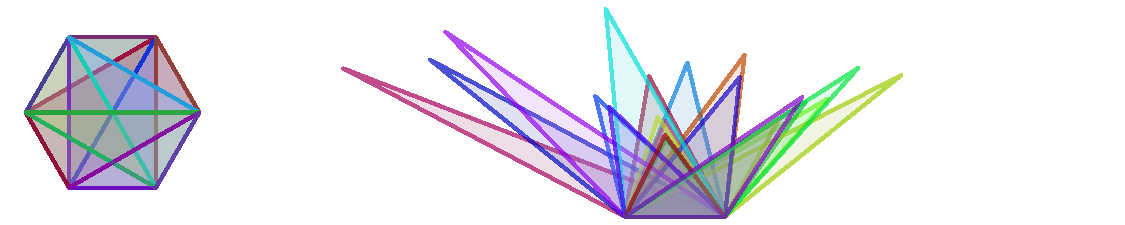
\includegraphics[width=1\textwidth]{R/tri1.pdf}
\caption{A given number of cliques can overlap maximally (left),
or not overlap much (right).}
\label{fig:overlappingTriangles}
\end{figure}

Triangles can be detected using matrix multiplication \cite{itai_finding_1977},
and there are fast algorithms known for matrix multiplication
\cite{strassen_gaussian_1969}
\cite{williams_multiplying_2012}, so the set of all possible
cliques on some set of vertices (Figure \ref{fig:overlappingTriangles}, left)
 can be detected
using fewer than one NAND gate per triangle (for large enough input graphs).

On the other hand, if the triangles overlap less (as in
Figure \ref{fig:overlappingTriangles}, right),
then to detect all of the triangles, we will definitely need at least one
gate per triangle. We can see this by feeding in a 0 to some input
unique to a triangle, applying Theorem \ref{edgeZonking}, and repeating.

Consider the case of finding $k$-cliques on $n$ vertices.
Possibly the most na\"ive strategy in this case is to pick a vertex $v_1$,
and feed in 0's to edges, one at a time. We can repeat this
(zonking at least one NAND gate as we go), until there
$k-2$ edges remaining connected to $v_1$. At this point, $v_1$ can no
longer be part of a clique. We feed in 0's to those edges (with no
provable effect on the circuit size), and repeat with $v_2$...
This strategy is simple, but only gives a bound a bit lower than
the number of input edges.

\subsection{Defining levels of CLIQUE}

To me, it seems a reasonably intuitive guess that the hardness of
computing $BUGGYCLIQUE(A)$ should be somehow related to
$|A|$, which is simply the number of cliques it ``sees''.

\begin{defn}
\label{CLIQUE-level}
Assume $n, k$ are fixed. For any $l$ such that
$0 \le l \le |K|$, let $K_l$ be the set of all sets
with exactly $l$ cliques. 
\end{defn}

We abuse notation slightly, and write

\[
BUGGYCLIQUE(K_l) = \{ BUGGYCLIQUE(k) : k \in K_l \}
\]

\begin{prob}
\label{gatesPerLevel}
Consider graphs with $n$ vertices.
Let $0 \le i \le N$.
How many gates are required to find a subset of size $i$ of the possible $N$
cliques?

\end{prob}

(When $i=N$, this is asking about the circuit complexity of $k-CLIQUE$, a
well-studied open problem, to say the least...)

Does the counting bound
say anything about $E[|\bigC(BUGGYCLIQUE(K_l))|]$, for
some fixed $l$? Let $N = {n \choose k}$.
At the ``bottom'', there's only one $BUGGYCLIQUE(\emptyset)$
function, so the counting argument is useless.
In the ``middle'',
there are ${N \choose {N/2}}$ functions, and so the counting
argument gives a nontrivial lower bound for
$E[|\bigC(BUGGYCLIQUE(K_{N \choose {N/2}}))|]$ (although
without actually constructing even {\em one} difficult function!).
At the ``top'', again, there's only one $BUGGYCLIQUE(K) = k-CLIQUE$
function, so the counting argument is, once again, useless.

It would be nice if we could show that, as $l$ increases,
$E[|\bigC(BUGGYCLIQUE(K_l))|]$ also increases.
(This {\em seems} intuitive -- if finding {\em half} of the cliques
is hard, at least sometimes, how much easier can finding {\em all}
of them be? But that's only intuition, not proof.)
If we could prove something in general, for all levels $l$, then at
the top of the diagram, we'd be bounding just the function
$BUGGYCLIQUE(K_l) = k-CLIQUE$. (This suggests that doing so would
be difficult...)

\section{Using random restrictions}

Random restrictions have been used in lower bounds of formula
\cite{subbotovskaya1963comparison} and circuit \cite{hastad1987lower}
complexity (see also the slides at \cite{rossmanRestrictions}).
Here, we apply random restrictions to a set of functions (and circuits),
rather than just one function and circuit.

\subsection{Counting functions by their ``rank'' in a list}

This argument relies on measuring the size of a circuit,
for a given basis. (Here, we assume unbounded fan-in
NAND gates, but this doesn't seem crucial.)

\begin{defn}
\label{Rank}
For all $C \subseteq K$,
arrange all of the sets of cliques in nondecreasing order
of $|\bigC(BUGGYCLIQUE(C))|$ (using unbounded fan-in NAND gates,
breaking ties by some lexicographic order of circuits).

Let $A \subset K$. The {\em rank} of $A$, $rank(A)$, is the zero-based
index of $A$ in this list.
\end{defn}

If we can lower-bound $rank(A)$, then we should be able to translate
that into a
lower bound on $|\bigC(BUGGYCLIQUE(A))|$. (Possibly, if we
can only lower-bound $E[rank(A)]$, we may be able to get
a bound in terms of number of gates using Jensen's inequality?
Not clear.)

We can imagine a miles-long linear warehouse of chips with the minimal
circuit for each problem, sorted in terms of number of gates.
(Note that the above list only includes functions in $BUGGYCLIQUE$.
There are a {\em ton} of other functions (parity, primality, ``looks
sort of like a bitmap of a cat'', etc.), but ignoring
those should still leave a valid lower bound for the functions in $BUGGYCLIQUE$.)

\subsection{How much smaller are ``restricted'' circuits, on average?}

\begin{thm}
\label{vaguelyUpward}
Let $C \subseteq K$ be a set of cliques chosen uniformly at random
from $K$.

Let $a = {n-2 \choose k-2}$ (this is the number of $k$-cliques
intersecting a given edge).

Then there is a function $f: 2^K \rightarrow 2^K$ such that
\begin{itemize}

\item $E[|C| - |f(C)|] = a/2$

\item $E[rank(C) - rank(f(C))] \ge a/2$

\end{itemize}

\end{thm}
\begin{proof}

Pick a distinguished input edge $e$, and let $A \subseteq C$ be
the set of cliques in $C$ which include $e$, and $B \subseteq C$ be
the set of cliques in $C$ which don't include $e$.

We define $f(C) = B$.

Now, take the circuit computing $BUGGYCLIQUE(C)$, and
feed in a 0 to $e$. The resulting circuit computes
$BUGGYCLIQUE(B)$. Note that $A$ could contain anywhere
from 0 to $a$
cliques, so since $C$ is chosen uniformly at random,
$E[|A|] = a/2$.

Furthermore, $|\bigC(B)| \le |\bigC(C)|$, because feeding in
a zero to the circuit for $BUGGYCLIQUE(C)$ constructed a
(possibly non-optimal) circuit for $BUGGYCLIQUE(B)$.
Thus, $rank(B) \le rank(C)$.
This means that
$C$ is one of $a$ functions chosen uniformly at random,
and so, on average, there are $a/2$ circuits between $C$
and $B$, implying at least that large a difference in rank.

(Note that if $e$ ``misses'' all of the cliques in $C$, then $B = C$
and $rank(B) = rank(C)$. However, provided $e$ is in some clique in $C$,
then since we're feeding in a 0 to a NAND-gate circuit,
the inequality $rank(B) < rank(C)$ is strict.)

\end{proof}

In terms of the previous warehouse analogy, we can see that,
when an edge is disabled, the chip now has strictly fewer gates.
Perhaps the chip-maker spent their entire budget on designing the
optimal circuits, but then skimped on the wires connecting the chips?
In that case, assuming the missing wire is treated as a 0, the chip still
finds some cliques, and so might yet be sellable.
By construction of the warehouse, that means the faulty chip could be shifted,
on a giant conveyor belt,
toward the ``smaller'' (in number of gates) end of the warehouse.
That means that the corresponding set of cliques is also
in the ``smaller'' end of the warehouse.

Note that these numbers both decrease, but not necessarily at the same rate.
The expected reduction in the number of cliques is $a/2$; I'm not sure
about the expected reduction in rank. Presumably near the middle, the
average rank will decrease a lot.

\subsubsection{Why this doesn't bound $k-CLIQUE$?}

\ref{vaguelyUpward} seems to show that ``finding more cliques is
at least a tiny bit harder on average.'' However, it only applies
on average.

\subsection{Estimating the rank of functions, at each level}

It seems intuitive that finding a larger fraction of the cliques
should be harder.
So, another idea is to try to show this using induction on $l$.
As usual, the base case ($l=0$) is easy: finding zero cliques is easiest,
so its rank is 0 (see Theorem \ref{zeroCliques}).

The step case is not so straightforward, though. Suppose we've computed bounds for
levels 0 through $l-1$ (thus, we're using some sort of strong induction.)
In other words, we've lower-bounded $E[rank(K_i)]$, for $i \in [0,l-1]$.
Can we lower-bound $E[rank(K_l)]$?
Suppose we pick a set of cliques at level $l$, uniformly at random.
If we then pick an edge $e$ uniformly at random, and remove the cliques
which contain $e$, then the number of cliques removed will vary
depending on the level. When $l=1$, we'll remove 0 or 1 cliques; when $l=N$,
we'll remove all ${n-2 \choose k-2}$ cliques which contain $e$.
The number of cliques ``hit'' will have a hypergeometric distribution,
which is relatively tractable.

However, unfortunately, the graphs which {\em remain} are no longer uniformly
sampled from each level! For instance, most levels include {\em tons} of
graphs which include all the input edges. The above procedure will not
be sampling any of them.

\subsection{Can we bound this using linear programming?}

We now attempt to bound the expected rank of finding a set
of cliques, as a function of the number of cliques.

This is implemented in
{\tt py/lp\_brute\_force\_1.py}. It uses a linear program, with
one variable $C_i$ per number of cliques, from 0 to ${n \choose k}$.
Each variable represents the average rank of the functions with
that many cliques.

\subsubsection{Some trivial rank upper bounds}

We start with a silly bound.

\begin{thm}
\label{zeroCliques}
Finding zero cliques has rank zero.
\end{thm}
\begin{proof}

Let $C$ be a circuit finding any non-empty set of cliques.
Feed in all 0's to $C$. It now finds zero cliques, and has
fewer gates. Thus, $C$ has more gates than the function
which finds zero cliques, and the rank of $C$ is greater
than zero.

Thus, the function finding zero cliques has rank zero.

\end{proof}
 
Another way of thinking of this is that ``all the other functions
are `above' finding zero cliques''.

This seems, in some sense, like using ``restrictions'' to prove an {\em upper} bound!
Also, it's non-constructive: it doesn't give any idea of what circuit finds no cliques
(although that's trivial); it only says that it must be easier than finding any
{\em other} set of cliques. (Alternatively, we could view this as using restrictions
to compute a lower bound -- on the average of $2^{n \choose k} - 1$ functions; which
is a bit uninformative.)

A slightly less silly example is that we can feed in zeros to 
the edges which hit all but $k$ vertices, leaving one clique.
We can do this in ${n \choose k}$ different ways. Thus, the rank
of all of these ways of finding exactly one clique, is right above
finding zero cliques.

Note the asymmetry of the situation. Using restrictions to show that
$CLIQUE$ has high rank is difficult, as $CLIQUE$ isn't ``higher'' than
many functions in $Z$. Each restriction step (corresponding to an edge in $Z$)
shows that a function is
``higher'', but only by some approximate amount.
On the other hand, at the other end of $Z$, we can unequivocally say
that {\em some} functions have low rank (and are thus
``relatively easy'' to compute).
This seems, at first, a trivial observation; we would expect upper bounds
to be easier to find than lower bounds. It also, at first, doesn't seem
to help in bounding the rank of $CLIQUE$.

However, recall that we know that the average rank of all the functions
is $N/2$.
When we show that the constant function has rank 0, that lifts
the average for all $N-1$ other functions (although admittedly
by a stunningly miniscule amount).
Similarly, the bound on finding one clique pushes up all the other functions.
Thus, perhaps, we can use such upper bounds to ``rule out'' $CLIQUE$ from
having low rank.

It's not clear, though, how well we can upper-bound the rank
of finding other sets of functions...

\subsubsection{Generalizing that upper bound}

Given a set $A$ of cliques, we
can find the set $E$ of edges which aren't present in any of those cliques.
Let $B$ be any clique which does include some edge in $E$, and let
$C = A \cup B$. If we feed in zeros to all edges to a circuit
finding the cliques in $C$, we end up with a strictly smaller circuit 
which finds the cliques in $A$.

Thus, for each level $i$, we loop through the sets of cliques in $C_i$.
For each set $A \in C_i$, we find the edges $E$ which aren't hit by any clique, and then
find $Z$, the set of cliques which {\em are} hit by an edge in $E$.
We then have that 

\[
rank(A) \le 2^{n \choose k} - 2^{|Z|}
\]

We compute an upper bound for every $A \in C_i$, and then average these
to get a bound on $rank(C_i)$. We use the fact that $C_i$ contains many
functions to sharpen the upper bound.

\[
E[rank(C_i)] \le 2^{n \choose k} - E[2^{|Z|}] - |C_i|/2
\]

This is implemented by {\tt add\_upper\_bound\_constraints}.

This has the {\em small practical problem} that it involves
looping over all $2^{n \choose k}$ functions. To reduce the computational
effort, rather than zeroing out individual edges,
we might zero out all edges incident to a vertex. This seems like it might reduce
the amount of bookkeeping, but presumably would only yield a weaker upper bound.

\subsubsection{Average constraints}

Another part of this strategy 
(implemented by {\tt add\_average\_rank\_constraint}) was
to use the average of all the functions:

\[
E[rank(A)] = (2^{n \choose k} - 1) / 2
\]

We also added a weak counting lower bound for each level $C_i$, of functions
with exactly $i$ cliques. (This latter bound, implemented by
{\tt add\_counting\_lower\_bounds}, only seemed to have much
effect for $0 < i < {n \choose k}/2$; data not shown.)

\[
E[rank(C_i)] \ge ({n \choose i} - 1) / 2
\]

\subsubsection{Results}

We set up the linear program, and asked it to minimize $E[C_{n \choose k}]$
(in other words, finding all the cliques). We ran this with $n=6$, $k=3$
(in other words, finding triangles in six-vertex graphs). In this case,
the possible ranks range from $0$ to $2^{6 \choose 3}-1 = 2^{20}-1 = 1,048,575$.
For each level, we get the following bounds:

\begin{verbatim}
level	bound
0	0.00
1	9.00
2	94.00
3	569.00
4	2421.50
5	7751.00
6	19379.00
7	38759.00
8	62984.00
9	83979.00
10	524306.40
11	964586.16
12	985586.57
13	1009813.80
14	1029194.80
15	1040823.27
16	1046152.95
17	1048005.50
18	1048480.50
19	1048565.50
20	0.00
\end{verbatim}

Circumstantially speaking, this approach seems to at least suggest
that finding {\em more than half} of the cliques is harder than finding
{\em fewer than half} of the cliques.

However, it fails to actually lower-bound $CLIQUE$.

\subsubsection{Further thoughts on this model}

Note that the above bound only used the structure of the lattice $Z$ 
(figure \ref{fig:Z}) to count gates ``above'' a given node.
Since we're using NAND gates, every edge along a path from $CLIQUE$ to $\emptyset$
implies a slightly smaller circuit. This doesn't, at first glance, help much, as
$CLIQUE$ (and all of the other functions) are at a height less than the number of edges
(in this example, 15).

One complication of this bound is that zeroing out an input edge leaves a potentially
irregular graph of input edges. If instead, we were to zero out all the edges incident to a
vertex $v$, then we simply end up with an input graph with one less vertex.
(And, similarly, we remove the cliques which include $v$ from consideration.)
This might simplify counting how many cliques ``remain'' at a given level.

We might also try counting gates instead of rank.
All of the functions, including $CLIQUE$, are only directly
``above'' a {\em tiny} fraction of the functions
in the lattice $Z$. However, possibly including the upper bound would force some
things intermediate between $CLIQUE$ and $\emptyset$ to have many gates.

\section{Related work}

This strategy relies heavily on a modification of Shannon's original
function-counting argument \cite{shannon_synthesis_1949},
combined with random restrictions
\cite{subbotovskaya1963comparison} \cite{hastad1987lower}.

A related question is whether problems
(such as $k$-SAT) are
hard on average \cite{bogdanov2006average}.
These efforts seem to focus more on whether
random
instances of a given problem are hard, rather
than using random problems to show that
a specific problem is hard.

This lower-bound strategy also seems potentially
relevant to quantum computing,
as the argument makes few restrictions on the sort of gates used.
However, we did use the property of NAND gates that ``feeding in
a 0 disables a gate''; it's not clear whether that's needed,
or holds for quantum gates.

\section{Conclusion}

We give a lower bound on finding {\em some} set of cliques.
It is a modified form of Shannon's counting argument
\cite{shannon_synthesis_1949}, combined with random restrictions
\cite{subbotovskaya1963comparison} \cite{hastad1987lower}.
This suggests {\em approximate} bounds on functions {\em similar} to $k$-CLIQUE.
Unfortunately, however, this is an approximate bound,
and so doesn't bound the complexity of $k$-CLIQUE.

If this worked, then by the contrapositive,
\cite{fenner1996complexity} would give a concise list of some of the consequences...

\section{Acknowledgements}

The author would like to thank William Gasarch for introducing him
to lower bound strategies, and probabilistic proofs.
He would also like to thank the maintainers of
several entertaining and relevant blogs, including but
not limited to: the Computational Complexity blog
(Lance Fortnow and William Gasarch), 
G\"odel's Lost Letter (Richard Lipton and Ken Regan),
and Shtetl-Optimized (Scott Aaronson). 

\bibliography{references}
\bibliographystyle{unsrt}

\end{document}

